\chapter{Setup and maintenance of the \ReplicaGenOne{}}\label{ch:replica-setup}

This chapter applies to the classic \ReplicaGenOne{} instrument panel shown in \autoref{fig:replica-classic}. If your dashboard matches the \ReplicaNextLong{} layout, refer to the previous chapter.

\begin{figure}[htbp]
    \centering
    \begin{subfigure}{0.46\textwidth}
        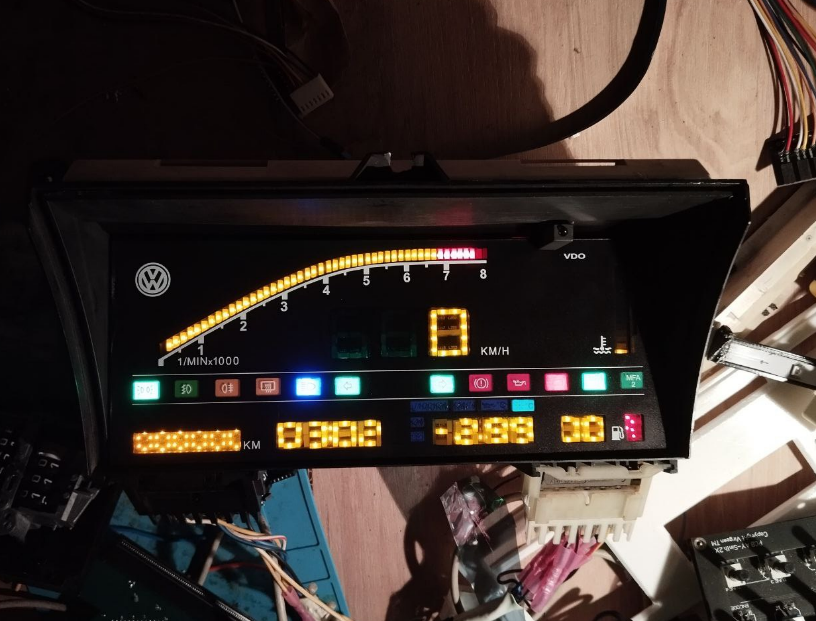
\includegraphics[width=\linewidth]{digifiz_manual/image046.png}
        \caption{Classic \ReplicaGenOne{} with square bezel.}
    \end{subfigure}\hfill
    \begin{subfigure}{0.46\textwidth}
        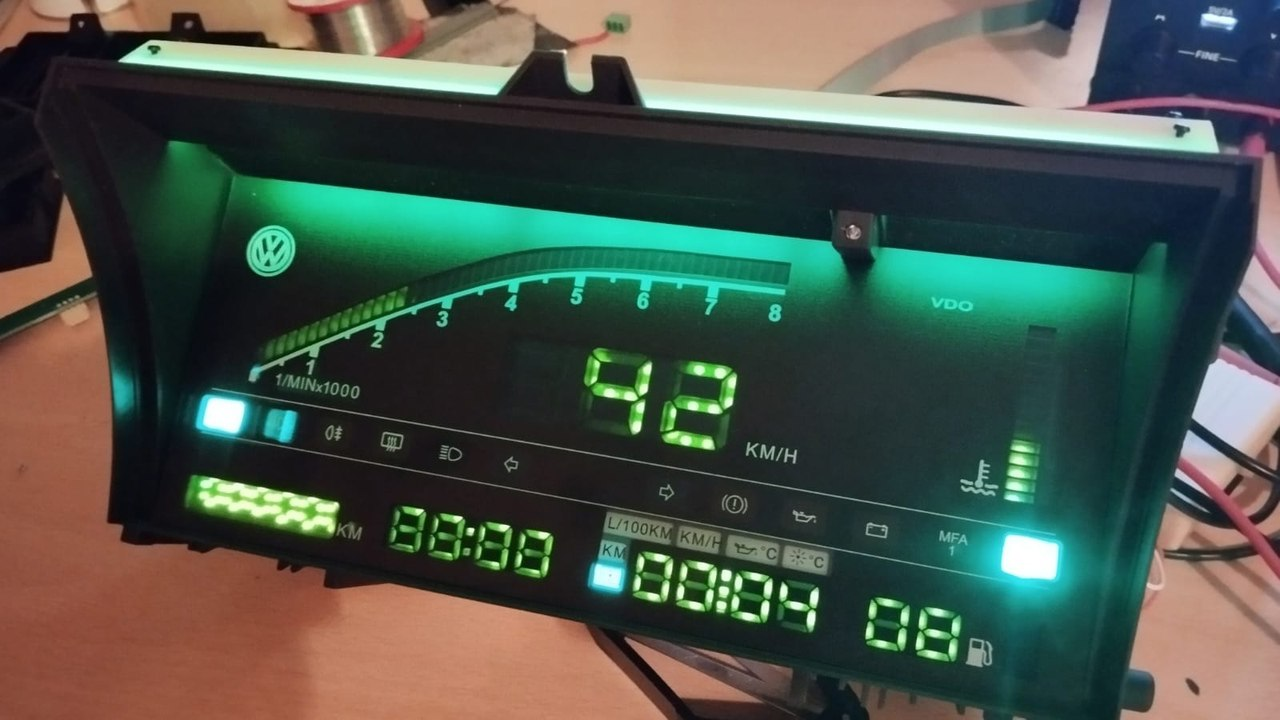
\includegraphics[width=\linewidth]{digifiz_manual/image047.png}
        \caption{Round-edge fascia used on later kits.}
    \end{subfigure}
    \caption{Appearance of the \ReplicaGenOne{} dashboard.}
    \label{fig:replica-classic}
\end{figure}

\section{Handling and screen care}
\begin{itemize}
    \item The plexiglass front with UV printing is easily marred. Avoid contact with sharp or abrasive objects.
    \item Surface damage is cosmetic and not covered by warranty. Request replacement parts from PHOL-LABS Kft if the screen pattern is deformed.
\end{itemize}

\section{Real-time clock battery}
The dashboard contains a DS3231 real-time clock with a CR2032 cell. The battery typically lasts about four years. When it is depleted the clock resets at every power-up. Remove the front and/or rear cover, keep the wiring harnesses connected, and replace the coin cell. Dispose of the spent battery according to local regulations.

\section{Firmware maintenance with USBasp}
Each kit ships with a USBasp programmer lead already connected inside the housing (\autoref{fig:usbasp-cable}). Install a suitable USBasp driver before flashing. For example, download it from the following address:
\displayurl{https://myrobot.ru/downloads/driver-usbasp-v-2.0-usb-isp-windows-7-8-10-xp.php}
The programmer powers the dashboard when it is connected to a computer, allowing bench checks.

\begin{figure}[htbp]
    \centering
    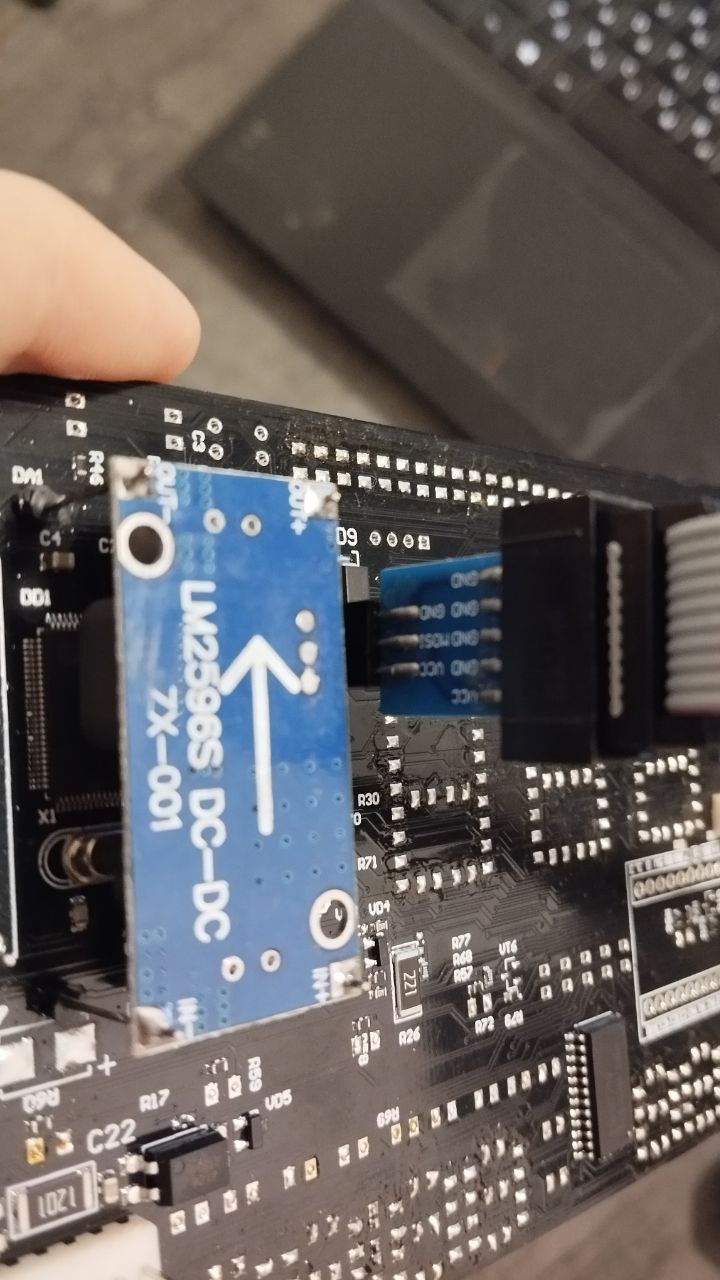
\includegraphics[width=0.32\textwidth]{digifiz_manual/image048.png}
    \caption{USBasp harness orientation inside the \ReplicaGenOne{}.}
    \label{fig:usbasp-cable}
\end{figure}

Flash firmware with \texttt{avrdude} using the command below (replace the firmware filename if required):

\begin{verbatim}
avrdude -c usbasp -p m2560 -e \
    -U lfuse:w:0xff:m -U hfuse:w:0x99:m -U efuse:w:0xff:m \
    -U flash:w:Digifiz.ino.mega.hex
\end{verbatim}

After a successful upload press the front touch button four to five times to initialise the memory blocks. If the blocks remain empty, repeat the flashing procedure or issue the Bluetooth command \verb|252 0| to trigger a factory reset. Ready-to-use firmware images are published at:
\displayurl{https://github.com/Sgw32/DigifizReplica}

\section{Bluetooth configuration}
Most parameters are adjusted over Bluetooth using an Android phone and the Serial Bluetooth Terminal application. Download it from the following link before pairing with the dashboard:
\displayurl{https://play.google.com/store/apps/details?id=de.kai_morich.serial_bluetooth_terminal&hl=en&gl=US}
iOS devices cannot connect to the classic Bluetooth 2.0 module.

\begin{itemize}
    \item Ensure you pair with the dashboard's Bluetooth Classic interface rather than BLE-only devices.
    \item In Serial Bluetooth Terminal set the end-of-line character to LF. Disable CR+LF before sending commands.
\end{itemize}

\begin{figure}[htbp]
    \centering
    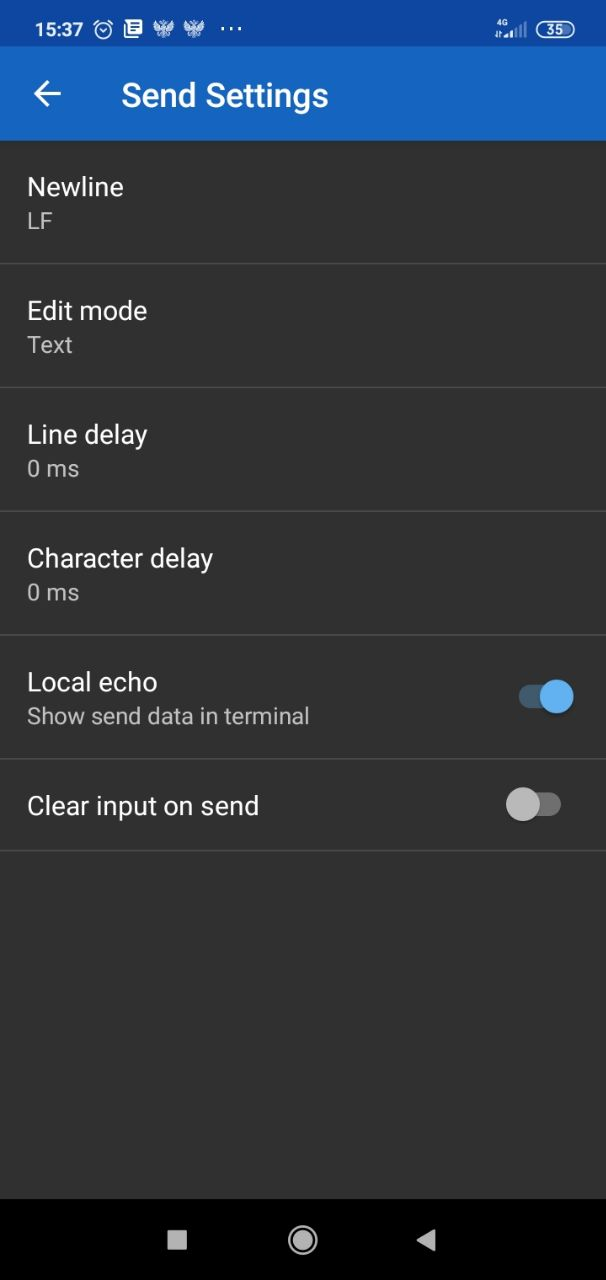
\includegraphics[width=0.32\textwidth]{digifiz_manual/image049.png}
    \caption{Recommended Serial Bluetooth Terminal configuration.}
    \label{fig:sbt-settings}
\end{figure}

Enter commands as space-separated pairs \verb|<number> <value>|. For example, to store an odometer value of 123\,456~km send \verb|11 123456|. Add 128 to a command number to read its current value (\verb|129 0| reports the speed coefficient). The diagnostic command \verb|adc 0| prints raw sensor readings that help the developers analyse faults.

\section{Configuration parameters}
The primary Bluetooth commands are listed in \autoref{tbl:replica-classic-commands}. Default settings for Generation~1/1.5 and Generation~2 dashboards are summarised in \autoref{tbl:replica-defaults}. Use commands~31--33 only on \ReplicaNextShort{} units; they have no effect on the classic \ReplicaGenOneShort{}.

{\scriptsize
\begin{longtblr}[
    caption = {Classic \ReplicaGenOne{} configuration commands.},
    label = {tbl:replica-classic-commands},
]{
    colspec = {Q[c,0.14\linewidth] >{\ttfamily}Q[l,0.38\linewidth] Q[l]},
    rowsep = 2pt,
}
    \toprule
    \textbf{ID} & \textbf{Name} & \textbf{Description} \\
    \midrule
    22 (or 0) & PARAMETER\_RPMCOEFFICIENT & Engine RPM calibration factor. \\
    1 & PARAMETER\_SPEEDCOEFFICIENT & Speed calibration factor. \\
    2 & PARAMETER\_COOLANTTHERMISTORB & Coolant thermistor beta coefficient. \\
    3 & PARAMETER\_OILTHERMISTORB & Oil thermistor beta coefficient. \\
    4 & PARAMETER\_AIRTHERMISTORB & Ambient thermistor beta coefficient. \\
    5 & PARAMETER\_TANKMINRESISTANCE & Minimum fuel sender resistance (\si{\ohm}). \\
    6 & PARAMETER\_TANKMAXRESISTANCE & Maximum fuel sender resistance (\si{\ohm}). \\
    7 & PARAMETER\_TAU\_COOLANT & Coolant temperature filter constant. \\
    8 & PARAMETER\_TAU\_OIL & Oil temperature filter constant. \\
    9 & PARAMETER\_TAU\_AIR & Ambient temperature filter constant. \\
    10 & PARAMETER\_TAU\_TANK & Fuel level filter constant. \\
    11 & PARAMETER\_MILEAGE & Total odometer value. \\
    12 & PARAMETER\_DAILY\_MILEAGE & Trip odometer. \\
    13 & PARAMETER\_AUTO\_BRIGHTNESS & Enable automatic brightness adjustment. \\
    14 & PARAMETER\_BRIGHTNESS\_LEVEL & Manual brightness level (0--15). \\
    15 & PARAMETER\_TANK\_CAPACITY & Fuel tank capacity (litres). \\
    16 & PARAMETER\_MFA\_STATE & Active MFA page. \\
    17 & PARAMETER\_BUZZER\_OFF & Disable the buzzer (1 disables, 0 enables). \\
    18 & PARAMETER\_MAX\_RPM & Tachometer scale (default 8000). \\
    19 & PARAMETER\_NORMAL\_RESISTANCE\_COOLANT & Coolant sensor resistance at \SI{25}{\celsius}. \\
    20 & PARAMETER\_NORMAL\_RESISTANCE\_OIL & Oil sensor resistance at \SI{25}{\celsius}. \\
    21 & PARAMETER\_NORMAL\_RESISTANCE\_AMB & Ambient sensor resistance at \SI{25}{\celsius}. \\
    23 & PARAMETER\_DOT\_OFF & Clock colon behaviour (0 blink, 1 solid). \\
    24 & PARAMETER\_BACKLIGHT\_ON & Switch on backlight with low beam. \\
    25 & PARAMETER\_M\_D\_FILTER & Median filter constant (legacy). \\
    26 & PARAMETER\_COOLANT\_MAX\_R & Coolant ``full-scale'' temperature threshold. \\
    27 & PARAMETER\_COOLANT\_MIN\_R & Coolant ``1~bar'' temperature threshold. \\
    31--33 & PARAMETER\_MAINCOLOR\_[RGB] & Interface colour components (\ReplicaNextShort{} only). \\
    37 & PARAMETER\_RPM\_FILTER & RPM filtering aggressiveness. \\
    128 & PARAMETER\_READ\_ADDITION & Add to read any parameter. \\
    255 & PARAMETER\_SET\_HOUR & Set clock hours (24-hour). \\
    254 & PARAMETER\_SET\_MINUTE & Set clock minutes. \\
    253 & PARAMETER\_RESET\_DAILY\_MILEAGE & Reset the trip odometer. \\
    252 & PARAMETER\_RESET\_DIGITAL & Factory reset and memory initialisation. \\
    \bottomrule
\end{longtblr}}

The Serial Bluetooth Terminal quick buttons are convenient for routine actions such as toggling automatic brightness (\verb|13 0| and \verb|13 1|) or writing colour values. Keep values above \SI{60}{\percent} brightness only for short tests to preserve LED life.
